\documentclass[a4paper,10pt]{article}

\usepackage[utf8]{inputenc}
\usepackage{tabularx}
\usepackage{csquotes}
% \usepackage[none]{hyphenat}
\usepackage[french=nohyphenation]{hyphsubst}
\usepackage{graphicx}
\usepackage{hyperref}
\usepackage{fancyhdr}
\usepackage{float}
\usepackage{caption}
\usepackage{listings}
\usepackage{spverbatim}
\usepackage{xcolor}
\usepackage[backend=bibtex]{biblatex}
\usepackage[toc]{glossaries}
\usepackage{wrapfig}
\usepackage{amsmath}
\usepackage[french]{babel}

\captionsetup{justification=centering}

\lstdefinestyle{customc}{
  belowcaptionskip=1\baselineskip,
  breaklines=true,
  frame=L,
  xleftmargin=\parindent,
  language=C,
  showstringspaces=false,
  basicstyle=\footnotesize\ttfamily,
  keywordstyle=\bfseries\color{green!40!black},
  commentstyle=\itshape\color{purple!40!black},
  identifierstyle=\color{blue},
  stringstyle=\color{orange},
}

\lstdefinestyle{customasm}{
  belowcaptionskip=1\baselineskip,
  frame=L,
  xleftmargin=\parindent,
  language=[x86masm]Assembler,
  basicstyle=\footnotesize\ttfamily,
  commentstyle=\itshape\color{purple!40!black},
}

\lstdefinestyle{custombash}{
  belowcaptionskip=1\baselineskip,
  breaklines=true,
  frame=L,
  xleftmargin=\parindent,
  language=bash,
  showstringspaces=false,
  basicstyle=\footnotesize\ttfamily,
}

\lstset{escapechar=@}

\rhead{BAUDVIN PUISSANT}
\chead{}
\lhead{TP-ECC-2015-2016}

\pagestyle{fancy}

\sloppy

\addbibresource{biblio.bib}
\include{glossary}



\begin{document}

%\maketitle
\begin{titlepage}
      \begin{center}   
        \Huge
        \textbf{Information theory}
        
        %\vspace{0.5cm}
        \LARGE
        ~
        
%         \vspace{0.5cm}
        
        \vfill
        \begin{figure}[H]
	    \centering
	    \begin{minipage}{0.89\textwidth}
		\centering
		
\includegraphics[width=\textwidth]{./img/esiea.jpeg}
	    \end{minipage}
	\end{figure}
        \vfill
        
        \vspace{0.5cm}
        
        TP de brute-force
        
        \vspace{2cm}
        \textbf{Emmanuel BAUDVIN\\Antoine PUISSANT}\\
        \vspace{0.8cm}
        \Large
        \underline{Enseignant :} M. FILIOL\\
        \vspace{0.5cm}
        2015 - 2016%\today
        
    \end{center}
\end{titlepage}

\begin{abstract}
L'objectif de ce mini-projet est de découvrir une application de la théorie des graphes dans le domaine de la sécurité. Vous allez étudier le problème MCS (Minimum Cut Set ou coupure minimale d'un graphe) dans le contexte du contrôle de zone. Ce dernier peut être envisagé de manière duale :
\begin{itemize}
 \item dans le cas défensif, il s'agit de protéger optimalement une zone donnée et ce, avec des ressources les plus limitées possibles,
 \item dans le cas offensif, par exemple, retarder, dans les mêmes conditions (optimalement et avec des ressources limitées), l'arrivée des forces d'intervention face à une attaque sur une zone donnée (point sensible)
\end{itemize}
\end{abstract}

\newpage

\tableofcontents

\section{Code de base}

\section{Question 2}
\textit{Etudiez l'algorithme de Ford-Fulkerson pour résoudre le problème du flot maximal. Décrivez-en le principe et les principales étapes algorithmiques.}\\
Dans cette partie nous allons étudier l’algorithme de Ford-Fulkerson, l’écrire en pseudo code puis expliciter chacune des étapes pour en comprendre le fonctionnement.\\
L'algorithme de Ford-Fulkerson (noté FF dans cette partie) est un algorithme qui permet de résoudre le problème du flot maximum dans un flot à une entrée et une sortie. Chacun des ces paramètres sont représentés sous la forme de nœud, structure classique des graphes qui sont reliés par des arcs. L’algorithme FF permet d'optimiser les flux dans les réseaux qui sont représentables dans les graphes (d'où le rapport entre le document et son application).\\
Ci-desous le pseudo code de l'algorithme:\\
Les entrées:\begin{itemize}
\item Un graphe G de capacité \textit{c}, noeud de départ \textit{s} et arrivé \textit{t};
\end{itemize}
Les sorties:\begin{itemize}
\item Une flux minimum entre \textit{s} et \textit{t}
\end{itemize}
\textbf{Algorithme \textit{Ford-Fulkerson}}
\begin{enumerate}
\item $f(u,v) \leftarrow 0$ \\ On met le poids des arcs à 0 pour tous les couples $(u,v)$; u et v étant des noeuds appartenant au graphe G.
\item \textbf{Tantque}($p=$ExisteUnChemin(s,t) \& capacité(u,v) $> 0$) \textbf{alors}\\
On itère alors des instructions en s'assurant que la capacité entre les noeuds u et v où l'on se situe permet de faire passer le dit flux dans le graphe. On vérifie aussi que le chemin entre s et t existe toujours.
\begin{itemize}
\item Chercher(capacité\_min(p))\\
On cherche alors la capacité minimale de p, le chemin entre s et t.
\item \textbf{PourChaque} $(u,v)\in p$ \textbf{faire}
\begin{itemize}
\item $f(u,v) \leftarrow f(u,v) + capacite(p)$\\
On envoie le flux à travers le graphe et on met à jour les poids des arcs
\item $f(v,u) \leftarrow f(v,u) - capacite(p)$\\
Cette instruction n'est là que si retourner la valeur du flux minimum à travers le graphe est nécessaire
\end{itemize}
\textbf{fin\_PourChaque}
\end{itemize}
\textbf{fin\_Tantque}
\end{enumerate}

\section{Question 3}
\textit{Expliquez le principe de résolution du problème MCS par l'algorithme de Ford-Fulkerson.}\\~\\\par
On peut résoudre le Minimum Cut Set Problem par l'algorithme de Ford Fulkerson grâce au théorème suivant :\\\par
Si \textit{f} est un flot dans un grpahe \textit{G}, les trois propositions suivantes sont équivalentes :\\
\begin{itemize}
 \item \textit{f} est un flot maximum (à fortiori, il le sera si on le calculle avec l'algorithme de Ford Fulkerson
 \item Le réseau résiduel du grpahe \textit{G} ne contient pas de chemin améliorant (puisqu'on aura appliqué Ford Fulkerson)
 \item Il existe une coupe du graphe \textit{G} séparant \textit{s} et \textit{t} dans deux sous graphes, dont la capacité vaut |\textit{f}|
\end{itemize}


\section{Question 4}
\textit{Décrivez et expliquez les principaux résultats de la référence \cite{tiquette} et comment les auteurs ont résolus le problème du contrôle de zone via l'algorithme de Ford-Fulkerson.}\\~\\\par
L'article donné en référence pour ce projet est à propos d'une étude réalisée par cinq chercheurs aux État-Unis. Cette dernière consiste en l'identification de postes de contrôles afin de protéger les grandes villes américaines.\\
Afin de trouver les localisions optimales des points de contrôle, les chercheurs ont trouvés plusieurs approches. Cependant, celle retenue consiste à chercher les points de contrôles minimum permettant de sécuriser la région choisie. Cet ensemble de points de contrôle est le appelé Minimum Cut Set (MCS) en théorie des graphes. En effet, nous pouvons représenter la ville à protéger par un graphe. Les liens seraient alors la représentation des axes de circulation et les nœuds les intersections entre plusieurs axes (un changement d'état pour un axe). Ainsi, le MCS permet de réaliser une coupe du graphe en deux parties disjointes.\\
Dans notre cas, nous souhaitons avoir le moins de liens à couper afin de ne mettre en place que des points de contrôles stratégiques. Ce problème peut être résolu par l'algorithme de flux maximum de Ford-Fulkerson.\\
Dans le cadre de cette étude, il ne sera pas pris en compte le coût des points de contrôle qui pourront être mis en place.\\
Tout au long de cet article, les chercheurs se sont focalisés sur les 50 plus grandes villes américaines (c.f. annexe \ref{annexe:1}).\\~\\\par
Dans un premier temps, il est nécessaire de définir deux variables que nous allons réutiliser tout au long de cette explication :
\begin{itemize}
 \item $r_i$, le rayon interne. Celui-ci définie la zone que nous souhaitons protéger. Si un acteur malveillant parvient à rentrer au sein de cette zone, alors nous devons considérer cette dernière comme perdue.
 \item $r_o$, le rayon externe. Celui-ci va correspondre à la zone au sein de laquelle nous allons effectuer nos contrôles.
\end{itemize}
Nous avons ici un système de cercles concentriques. Le cercle interne doit avoir un rayon $r_i$ inférieur ou égal à celui du cercle externe, $r_o$ comme le montre l'image \ref{img:1}. On a ici un rayon interne $r_i$ de $15$ miles ($\approx 24km$) et in rayon externe $r_o$ de $25$ miles ($\approx 40km$).
\begin{figure}[H]
 \centering
 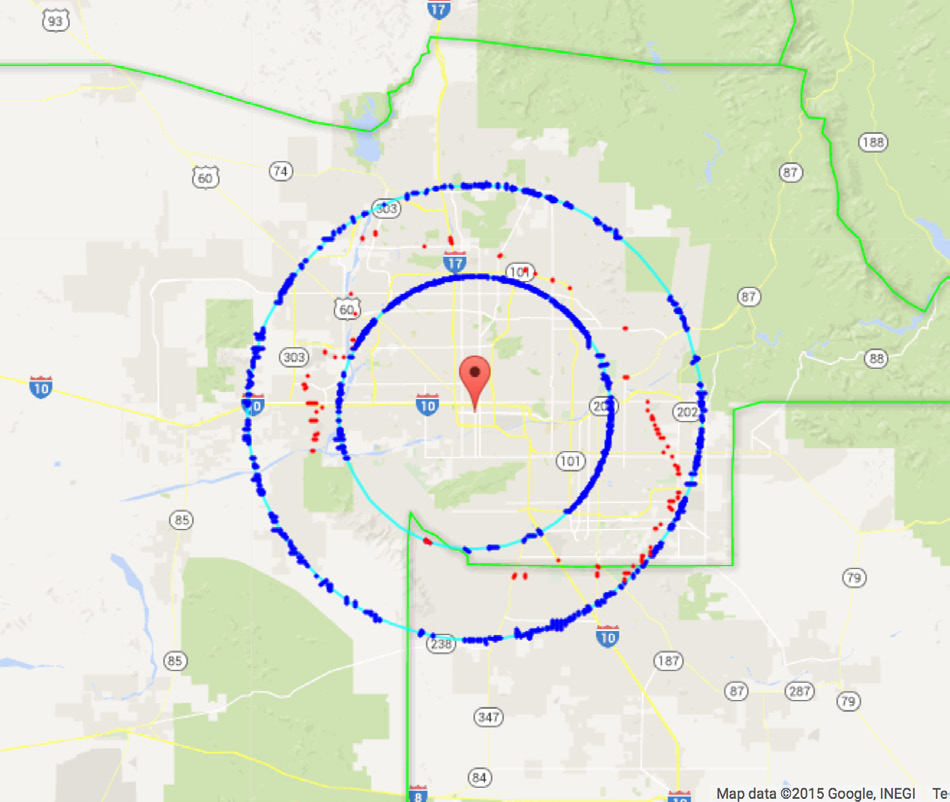
\includegraphics[width=.5\textwidth]{img/circles.png}
 \caption{Représentation des cercles interne et externe pour la ville de Phoenix}
 \label{img:1}
\end{figure}
Ainsi, la zone présente entre les deux cercles peut être qualifiée de \enquote{zone tampon}. C'est au sein de cette dernière que nous allons placer les points de contrôle.\\
Sur l'image \ref{img:1}, nous pouvons retrouver différentes notations :
\begin{itemize}
 \item En bleu clair sont représentés les cercles internes et externes.
 \item En bleu foncé sont représentés les axes et routes s'intersectant avec les cercles.
 \item En rouge sont représentés les routes appartenant à la MCS.
\end{itemize}
Dans notre exemple, nous avons la taille de la MCS, $M(15,25)=64$. Ainsi, nous savons qu'il faudra, en suivant cette configuration 64 points de contrôle afin de pouvoir protéger la zone interne.\\
Si nous prenons un cercle externe plus grand, nous pouvons constater que le nombre de points de contrôle va alors varier :
\begin{figure}[H]
 \centering
 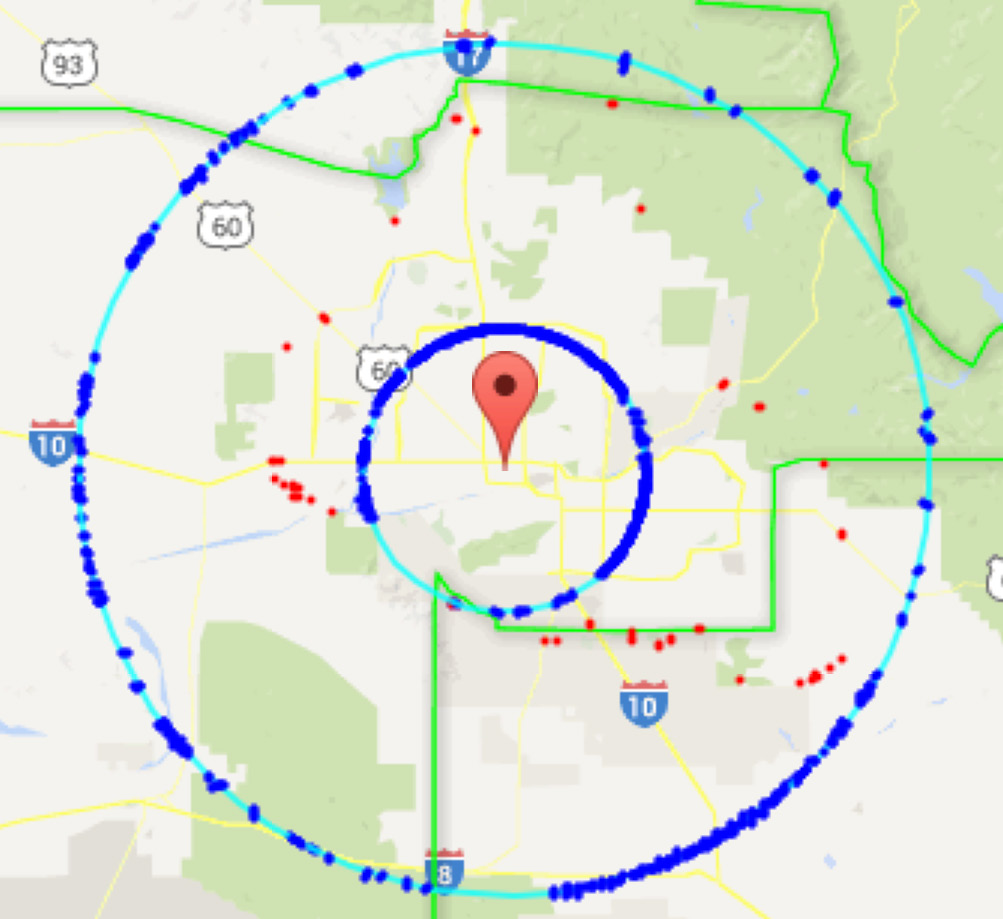
\includegraphics[width=.5\textwidth]{img/circles2.png}
 \caption{Représentation des cercles interne et externe pour la ville de Phoenix avec une MCS $(15,45)$}
 \label{img:2}
\end{figure}
Ici, nous sommes dans une configuration $(15,45)$. Ainsi, nous avons une zone tampon beaucoup plus grande que dans l'exemple précédent. Ainsi, le nombre de points de contrôle va logiquement varier. En effet, en agrandissant la zone tampon, le nombre de routes va changer. Ainsi, nous avons dans notre configuration moins de petits axes coupant notre zone. La proportion de grands axes va alors faire diminuer le nombre de points de contrôles à 36.\\
Ainsi, un des premiers résultats que l'étude permet de montrer est la relation entre la zone tampon et le nombre de points de contrôle nécessaires à la protection de la zone. Afin de définir quel est le meilleur couple de variables pour chacune des villes, l'étude s'est focalisée sur trois tailles de cercles internes $r_i$ : $5$, $10$ et $15$ miles. Il est ainsi possible de regrouper les différentes villes grâce au regroupement $k$-moyen.\\
En suivant ces règles, et en définissant $r_o$ à $45$ miles, les chercheurs ont pu comparer les résultats obtenus pour les différentes villes. Nous pouvons retrouver sur l'image \ref{img:3} la distribution des tailles des MCS pour un couple de zones $M(15,45)$.
\begin{figure}[H]
 \centering
 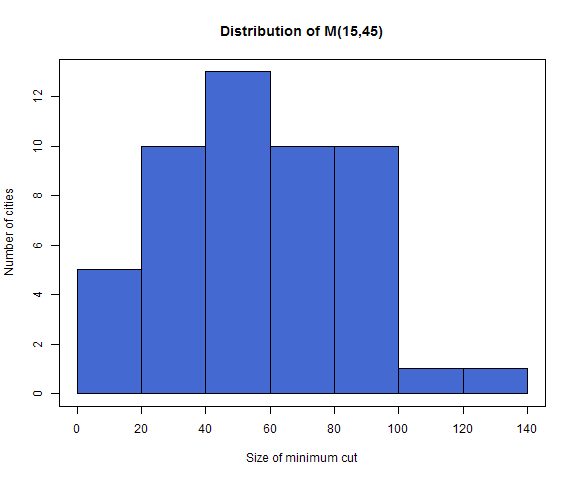
\includegraphics[width=.7\textwidth]{img/histo.png}
 \caption{Distribution des tailles de MCS pour $M(15,45)$}
 \label{img:3}
\end{figure}
On remarque alors que la taille médiane de la coupe est de $55,5$. Ces coupes sont majorées par la coupe de Philadelphie ($124$) et minorée par celle de Las Vegas ($10$). Nous expliquerons plus tard en quoi une aussi grande variation a lieu.\\
Les chercheurs se sont ici attardé sur une des coupes pour le système $M(15,45)$. En effet, en étudiant les différentes possibilités de zone tampon, ils se sont rendu compte qu'il était possible de réduire la taille de la coupe MCS jusqu'à $95\%$ en augmentant la zone. En effet, si l'on observe les résultats reportés dans le tableau \ref{tab:1}, nous pouvons remarquer que la taille des MCS de chaque ville diminue en passant de $M(15,15)$ à $M(15,45)$.
\begin{table}[H]
 \centering
 \begin{tabular}{|l|c|c|c|}
    \toprule
    \textbf{Ville} & \textbf{$M(15,15)$} & \textbf{$M(15,45)$} & \textbf{MCS réduction}\\\midrule
    Miami & 309 & 16 & $95\%$ \\\hline
    Virginia Beach & 167 & 10 & $94\%$ \\\hline
    Los Angeles & 650 & 61 & $91\%$ \\\hline
    New York City & 759 & 87 & $89\%$ \\\hline
    Atlanta & 478 & 98 & $79\%$ \\\hline
    Indianapolis & 293 & 107 & $63\%$ \\\hline
    Oklahoma City & 215 & 91 & $62\%$ \\\hline
    Columbus & 188 & 91 & $52\%$ \\\bottomrule
 \end{tabular}
 \caption{Diminution de la taille des MCS en augmentant de 30 miles la zone tampon}
 \label{tab:1}
\end{table}
Cela s'explique du fait que plus nous sommes proche du centre des villes, plus le nombre d'axes routiers est important. En effet, en pouvant effectuer les contrôles sur une zone plus large, les axes des villes se regroupent en de plus grands axes. Il est alors plus simple de réduire le nombre de points de contrôle sur ces grands axes. Les réductions sont plus où moins grandes en fonction de la position géographique des villes. En effet, pour des villes comme Columbus ou Oklahoma City, il n'y a aucune barrière naturelle. Ainsi de axes routiers viennent de tout part autour de ces dernières. Cependant, pour des villes comme Miami ou Virginia Beach, la règle opposée s'applique. En effet, Miami possède des barrières naturelles (l'océan Atlantique à l'Est, les Everglades à l'Ouest, le Golfe du Mexique au Sud). Il n'existe alors que peu d'axes routiers, permettant un contrôle total de la circulation avec un minimum de points de contrôle.\\
Si l'on reproduit ce procédé en changeant la taille du cercle interne (5, 10 ou 15 miles), on se rend compte qu'à partir d'une certaine taille de la zone tampon (augmentation du cercle externe), la taille du MCS se stabilise, et cela peu importe la position géographique de la ville ou la taille du cercle interne.\\
On peut alors noter que la réduction de la taille du MCS est effectuée assez rapidement. Il n'est pas nécessaire d'augmenter la taille de la zone tampon de manière trop importante pour obtenir de très bons résultats. Pour un cercle externe, $r_o=30$ miles, pour plus de 45 villes la taille de la MCS est $64\%$ plus petite que le cas $M(15,15)$.\\~\\\par
Afin de pouvoir réaliser un modèle pouvant s'appliquer à plus de villes, les chercheurs ont voulu regrouper les villes étudiées en différents groupes en fonction de la taille de leur MCS. Ils ont pour cela utilisé l'algorithme du $k-$moyen. On retrouve alors quatre groupes :
\begin{itemize}
 \item Le premier regroupe des villes ayant un MCS très petit. De manière générale, ces villes sont protégées par des barrières naturelles et ne sont alors qu'accessible que par peu de routes.
 \item Les groupes deux et trois sont assez similaire. On y retrouve des villes dont le MCS minimum est rapidement atteint lors de l'augmentation de la zone tampon.
 \item Enfin, le dernier groupe rassemble quand à lui les villes au MCS le plus grand. Pour la majeure partie de ces villes, il n'y a pas de barrière naturelle et de nombreux axes routiers arrivent de part et d'autre. Elles ont des réseaux routiers beaucoup plus important que les autres villes.
\end{itemize}
Cependant, ce regroupement ne permet pas d'établir un modèle parfait, mais une approximation des moyens qui seront à mettre en place pour les villes.\\~\\\par
Afin de réaliser une analyse de coût de leur solution, les chercheurs on alors sélectionné une ville de chaque groupe :
\begin{enumerate}
 \item San Francisco
 \item Austin
 \item New York City
 \item Philadelphie
\end{enumerate}
Le but de cette démarche est de connaître le nombre de points de contrôle nécessaires en fonction de la taille de la zone à protéger. Pour ce faire, ils ont fixé $r_o=45$. On peut alors retrouver la taille des MCS dans le tableau \ref{tab:2}.
\begin{table}[H]
 \centering
 \begin{tabular}{|l|c|c|c|c|c|}
    \toprule
    \textbf{Ville} & \textbf{$M(5,45)$} & \textbf{$M(15,45)$} & \textbf{$M(25,45)$} & \textbf{$M(35,45)$} & \textbf{$M(40,45)$}\\\midrule
    San Francisco & 17 & 39 & 46 & 84 & 95\\\hline
    Austin & 33 & 46 & 65 & 88 & 109\\\hline
    New York City & 46 & 87 & 109 & 128 & 168\\\hline
    Philadelphie & 88 & 124 & 143 & 177 & 204\\\bottomrule
 \end{tabular}
 \caption{Nombre total des points de contrôle pour les villes représentatives}
 \label{tab:2}
\end{table}
Grâce à ces calculs, on se rend rapidement compte qu'il est possible de protéger une plus grande zone avec le même nombre de point de contrôle (83 points de contrôle pour protéger 8 ou 12 miles de New York City). Ce n'est cependant pas le cas de toutes les villes puisque pour Austin ou Philadelphie, l'augmentation du nombre de points de contrôle se fait à chaque augmentation de la taille de la zone à protéger.\\~\\~\\\par
Pour conclure, nous pouvons noter que les chercheur ont pu résoudre le problème du contrôle de zone grâce à l'algorithme de Ford-Fulkerson. En effet, en représentant les axes routiers de grandes villes comme des graphes, il leur a été possible de déterminer un MCS de la zone, dont tous les points d'intersections représentent des points de contrôle. Leur étude à permis de mettre en évidence la relation entre la taille de la zone à protéger, la taille de la zone de contrôle, l'environnement géographique de la ville et le nombre de points de contrôle.\\
Cependant, dans cette démarche, tous les axes routiers avaient le même poids dans le graphe. Aucun axe n'est plus important qu'un autre. Il serait judicieux, pour mettre un modèle beaucoup plus efficace (permettant de savoir quel type de contrôle mettre en place à chaque point de contrôle) de pondérer les axes en fonction de leur taille, importance.

%  \newpage
% \rhead{2014-2015}
% \nocite{*}
% \printbibliography\addcontentsline{toc}{section}{Références}
% \newpage
% \glsaddall
% \printglossaries

%\listoffigures\addcontentsline{toc}{section}{\listfigurename}
\end{document}
